\documentclass{fancyslides} 
\usepackage[utf8]{inputenc}
\usepackage{times}

\usepackage{graphicx}
\usepackage{caption}
\usepackage{subcaption}
\usepackage{ragged2e} %paquete para justificar texto


\usepackage[backend=bibtex]{biblatex  }

\bibliography{bibliografia}
\graphicspath{{img/}}
\setbeamertemplate{bibliography item}[text]



%%% Beamer settings (do not change)
\usetheme{default} 
\setbeamertemplate{navigation symbols}{} %no navigation symbols
\setbeamercolor{structure}{fg=\yourowntexcol} 
\setbeamercolor{normal text}{fg=\yourowntexcol} 



%%%%%%%%%%%%%%%%%%%%%%%%%
%%% CUSTOMISATIONS %%%%%%
%%%%%%%%%%%%%%%%%%%%%%%%%


%%%% SLIDE ELEMENTS
\newcommand{\structureopacity}{0.75} %opacity for the structure elements (boxes and dots)
\newcommand{\strcolor}{orange} %elements colour (predefined blue; orange; green)

%%%% TEXT COLOUR
\newcommand{\yourowntexcol}{white}


%%%%%%%%%%%%%%%%%%%%%%%%%
%%% TITLE SLIDE DATA %%%%
%%%%%%%%%%%%%%%%%%%%%%%%%
\fbckg{fondo}
\newcommand{\titlephrase}{Herramientas y temáticas actuales de Data Warehouses y OLAP}
\newcommand{\name}{Javier Bonet \\ Joel Catacora \\}
\newcommand{\affil}{Base de datos avanzada}
\newcommand{\email}{13 de mayo del 2015}


\begin{document}


\startingslide %this generates titlepage from the data above

\fbckg{white}
\begin{frame}
\pointedsl{{\Large Temas en investigación}}
\end{frame}

\fbckg{white}
\begin{frame}
\misc
{
Estos son algunos tópicos que están en desarrollo, y que veremos rapidamente:
\begin{itemize}
  \item El diseño de un Data Warehouse (DW)
  \item Ontologías para el diseño de un Data Warehouse
  \item Data Warehouse espaciales
  \item Web Warehouse
  \item Fuzzy Data Warehouse
\end{itemize}
}
\end{frame}

\fbckg{white}
\begin{frame}
\pointedsl{{\Large Diseño general de un DW}}
\end{frame}

\fbckg{white}
\begin{frame}
\misc
{

 \justifying Este método, propuesto en \cite{VaismanZimanyi14}, se basa en la suposición de que los DWs son un tipo particular de bases de datos dedicado para fines analíticos. Por lo tanto, su diseño debe seguir las fases de diseño de bases de datos tradicionales, es decir, la especificación de los requisitos, diseño conceptual, diseño lógico y diseño físico. Sin embargo, hay diferencias significativas entre las fases del diseño de bases de una datos tradicional y un DW, que se derivan de su diferentes naturalezas.

\begin{center}
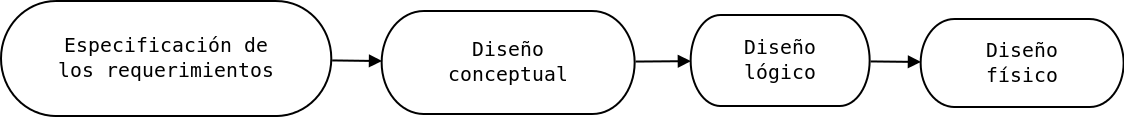
\includegraphics[scale=0.25]{diseno1}  
\end{center}

}
\end{frame}

\fbckg{white}
\begin{frame}
\misc
{

\begin{itemize}
  \item \textbf{Especificación de los requerimientos}: \justifying determina, entre otras cosas, \textit{que} datos deben estar disponibles y \textit{cómo} deben organizarse. 
  \item \textbf{Diseño conceptual}: \justifying la fase anterior debe proporcionar los elementos necesarios para la construcción de un esquema conceptual inicial del Data Warehouse.
  \item \textbf{Diseño lógico}: \justifying primero, consiste en la transformación del esquema conceptual en un esquema lógico; y segundo, la especificación de los procesos ETL.
  \item \textbf{Diseño físico}: \justifying abarca la implementación, tanto de los esquema del DW, como de los procesos ETL. Durante la fase de diseño físico, el esquema lógico se convierte en una estructura de base de datos física.
\end{itemize}

}
\end{frame}

\fbckg{white}
\begin{frame}
\pointedsl{{\Large Diseño conceptual}}
\end{frame}

\fbckg{white}
\begin{frame}
\misc
{
\justifying Siguiendo \cite{VaismanZimanyi14}, vamos a utilizar el modelo \textbf{MultiDim} para definir los esquemas conceptuales, aunque también se pueden utilizar otros modelos conceptuales que proporcionan una representación abstracta de un esquema del DW.
}
\end{frame}

\fbckg{white}
\begin{frame}
\misc
{
Presentamos los principales componentes del modelo:
\begin{itemize}
  \item \justifying Un \textbf{esquema} se compone de un conjunto de dimensiones y de un conjunto de hechos.
  \item \justifying Una \textbf{dimensión} se compone de un nivel o una o más je-rarquías.
  \item \justifying Una \textbf{jerarquía} está a su vez compuesto por un conjunto de niveles.
  \item \justifying Un \textbf{nivel} es análogo a una entidad en el modelo E/R.
  \item \justifying Un nivel tiene un conjunto de \textbf{atributos} que describen las características de sus miembros. Además, un nivel tiene uno o varios \textbf{identificadores}.
\end{itemize}
}
\end{frame}

\fbckg{white}
\begin{frame}
\misc
{
\begin{itemize}
  \item \justifying Un \textbf{hecho} relaciona varios niveles. El mismo nivel puede participar varias veces con un hecho, mediante diferentes \textbf{roles}.  Cada rol se identifica por un nombre.
  \item \justifying Un hecho puede contener atributos llamados \textbf{medidas}.
  \item \justifying Las medidas se sumarizan a largo de dimensiones cuando se realizan operaciones roll-up. La \textbf{función de sumarización} asociada con una medida se puede especificar junto al nombre de la medida; SUM por defecto.
  \item \justifying Podemos clasificar a las métricas como \textbf{aditiva}, \textbf{semiaditiva}, o \textbf{no aditiva}. Además, las medidas y los atributos de nivel puden \textbf{derivarse}, es decir que se calculan en base a otras medidas o atributos en el esquema. Por defecto, las medidas son aditivas.
\end{itemize}
}
\end{frame}

\fbckg{white}
\begin{frame}
\misc
{
Estas son algunas de las notaciones del modelo \textbf{MultiDim}.

\begin{center}
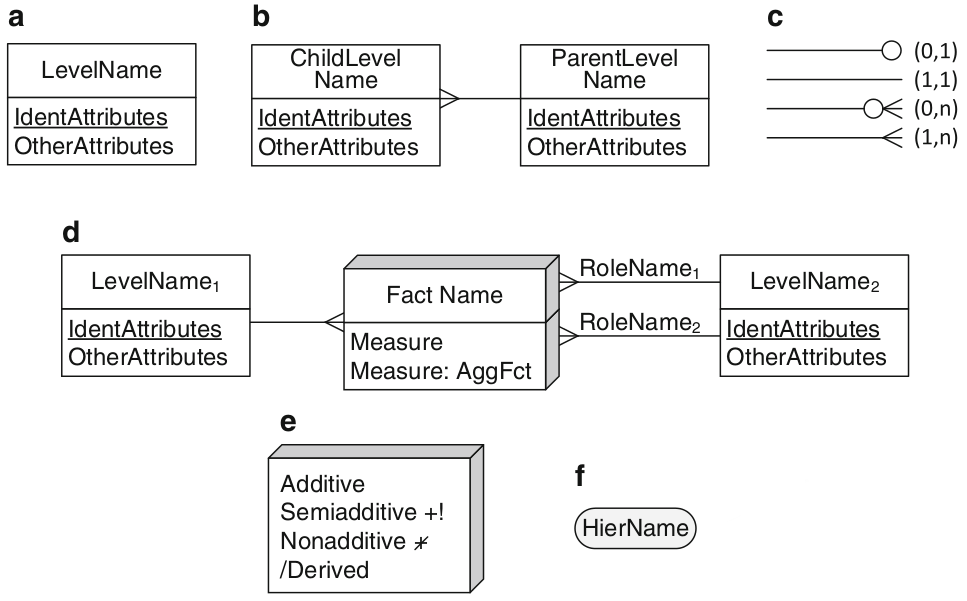
\includegraphics[scale=0.22]{diseno2}

{\footnotesize (a) Nivel, (b) jerarquía, (c) cardinalidades, (d) hecho con las medidas y niveles asociados, (e) tipos de medidas, (f) nombre de la jerarquía.}
\end{center}
}
\end{frame}


\fbckg{white}
\begin{frame}
\misc
{ \textbf{Ejemplo 1}:

\begin{center}
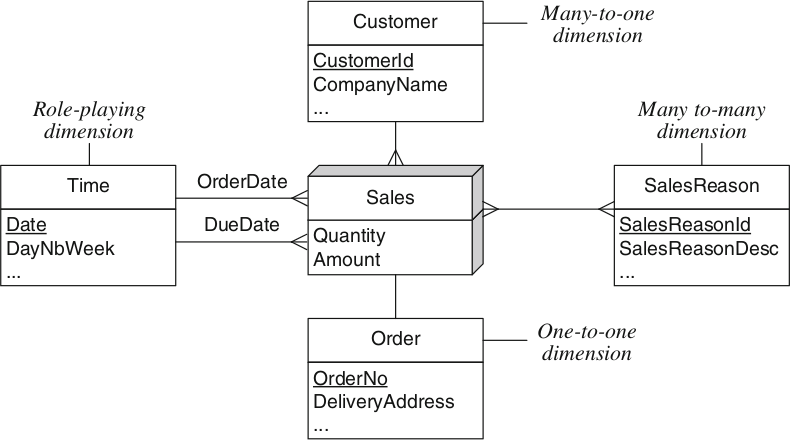
\includegraphics[scale=0.3]{diseno3}
\end{center}
}
\end{frame}

\fbckg{white}
\begin{frame}
\misc
{ 
\begin{center}
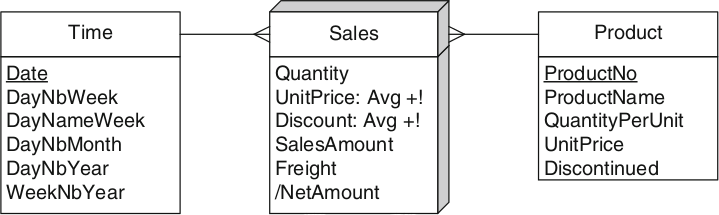
\includegraphics[scale=0.24]{diseno4}

\textbf{Ejemplo 2}
\vspace{2mm}

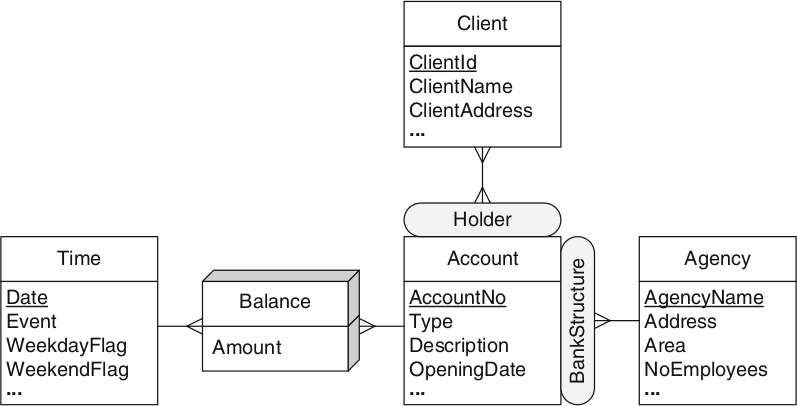
\includegraphics[scale=0.2]{diseno5}

\textbf{Ejemplo 3}
\end{center}
}
\end{frame}


\fbckg{white}
\begin{frame}
\pointedsl{{\Large Ontologías}}
\end{frame}

\fbckg{white}
\begin{frame}
\misc
{ 
\justifying La utilización y el análisis de datos no estructurados como pueden ser los archivos de texto, la web semántica, etc., han sido incluidos entre las posibles fuentes de datos, ya que presentan una gran cantidad de información que pueden aportar para la tarea de toma de desiciones.

}
\end{frame}

\fbckg{white}
\begin{frame}
\misc
{ \textbf{\Large Breve repaso de ontologías}
\newline
\newline

\justifying \textbf{Object property}: Son relaciones entre instancias de 2 clases. Por ejemplo, ownedBy, podría ser una object type property con la clase Vehículo como dominio y la clase Persona como rango.

\justifying \textbf{Data property}: Son como las object properties pero tienen como dominio una clase y rango un valor literal. Por ejemplo, si para una persona yo quisiera darle el nombre completo, entonces defino la data property fullName con dominio en Person y rango string.

\justifying \textbf{Individuals}: Representan los objetos o instancias de las clases que tenemos definidas en nuestra ontología.

}
\end{frame}


\fbckg{white}
\begin{frame}
\misc
{ \textbf{\Large Pasos a seguir para generar el DW}
\newline
\newline

\begin{itemize}
  \item \textbf{Creación de tablas a partir de las clases}.
\end{itemize}


}
\end{frame}

\fbckg{white}
\begin{frame}
\misc
{
\begin{center}
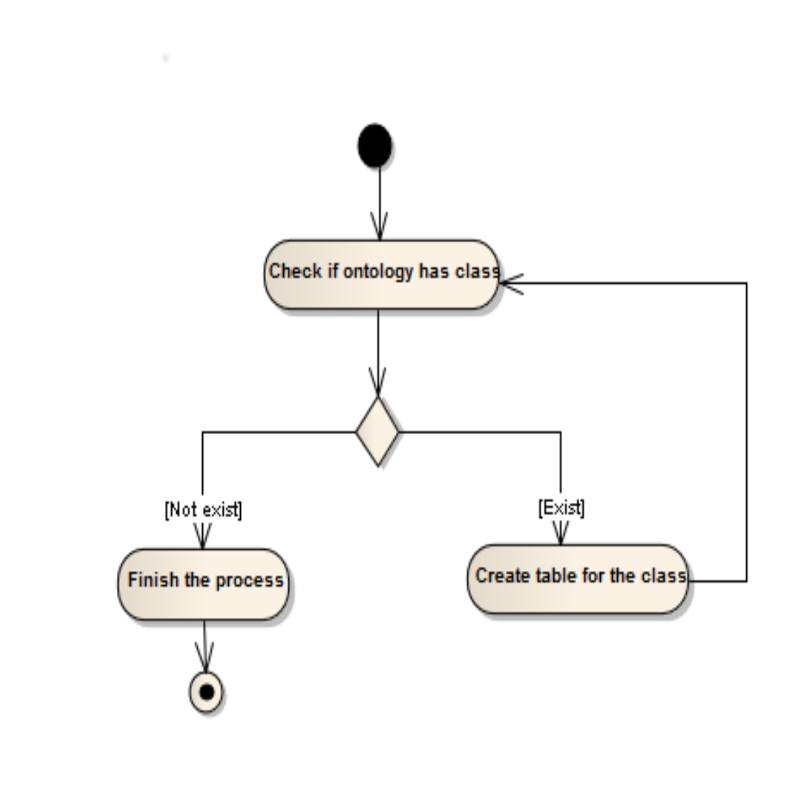
\includegraphics[scale=0.2]{create_tables}
\end{center}
}
\end{frame}


\fbckg{white}
\begin{frame}
\misc
{ \textbf{\Large Pasos a seguir para generar el DW}
\newline
\newline

\begin{itemize}
  \item \textbf{Creación de tablas a partir de las clases}.
  \item \textbf{Relaciones de subclase}.
\end{itemize}

}
\end{frame}

\fbckg{white}
\begin{frame}
\misc
{
\begin{center}
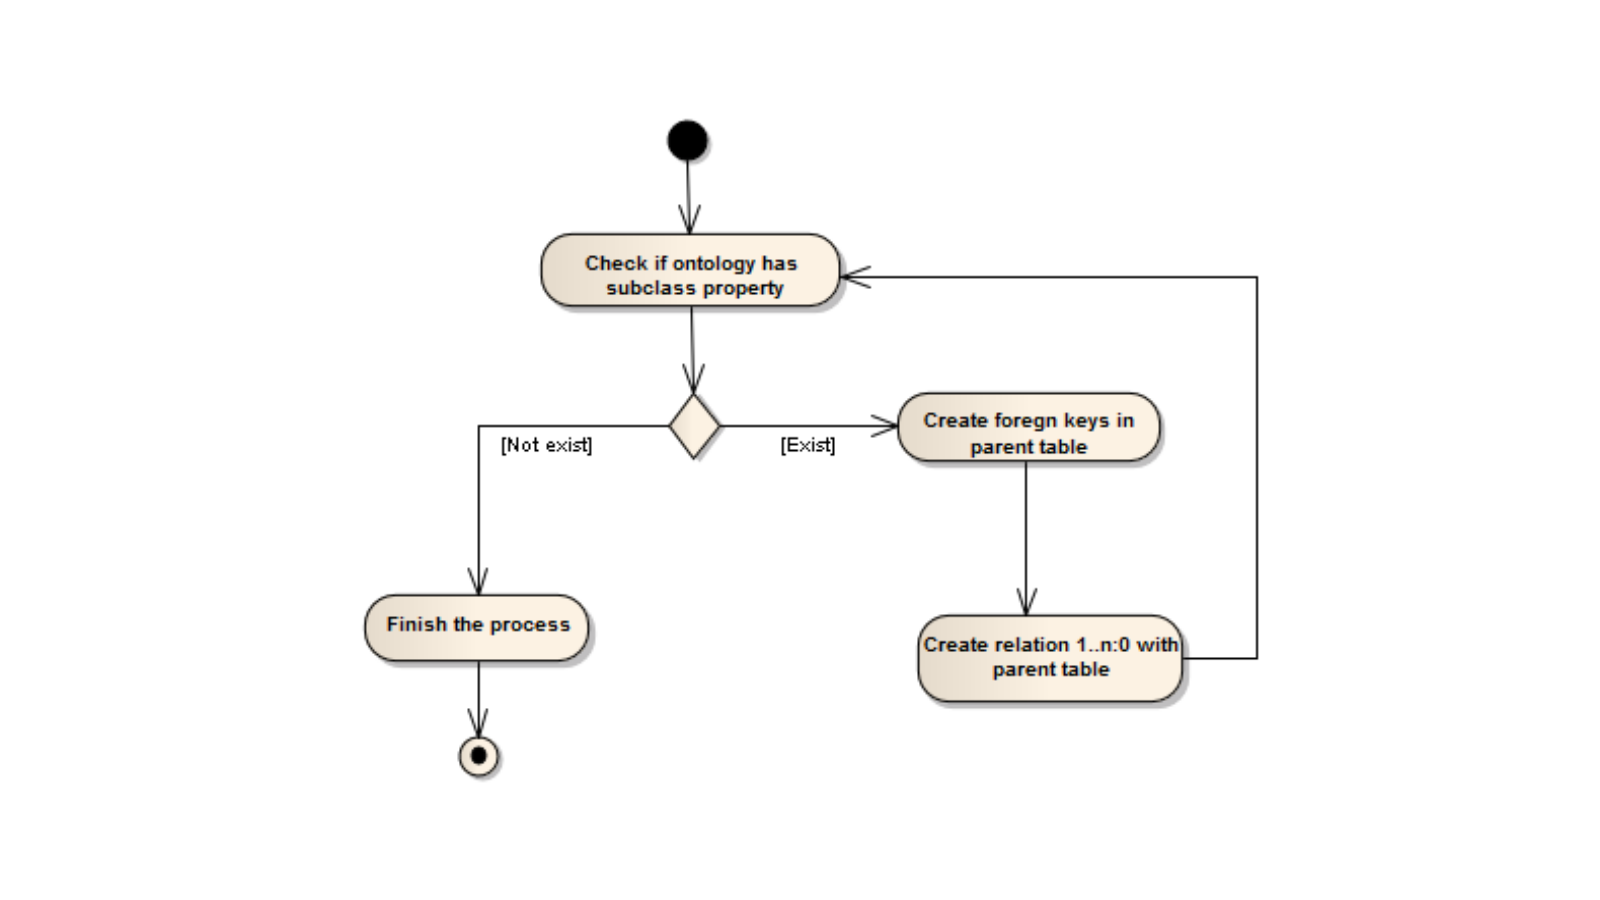
\includegraphics[scale=0.2]{is_a}
\end{center}
}
\end{frame}


\begin{frame}
\misc
{ \textbf{\Large Pasos a seguir para generar el DW}
\newline
\newline

\begin{itemize}
  \item \textbf{Creación de tablas a partir de las clases}.
  \item \textbf{Relaciones de subclase}.
  \item \textbf{Definiendo relaciones de propiedad de objetos}
\end{itemize}

}
\end{frame}

\fbckg{white}
\begin{frame}
\misc
{
\begin{center}
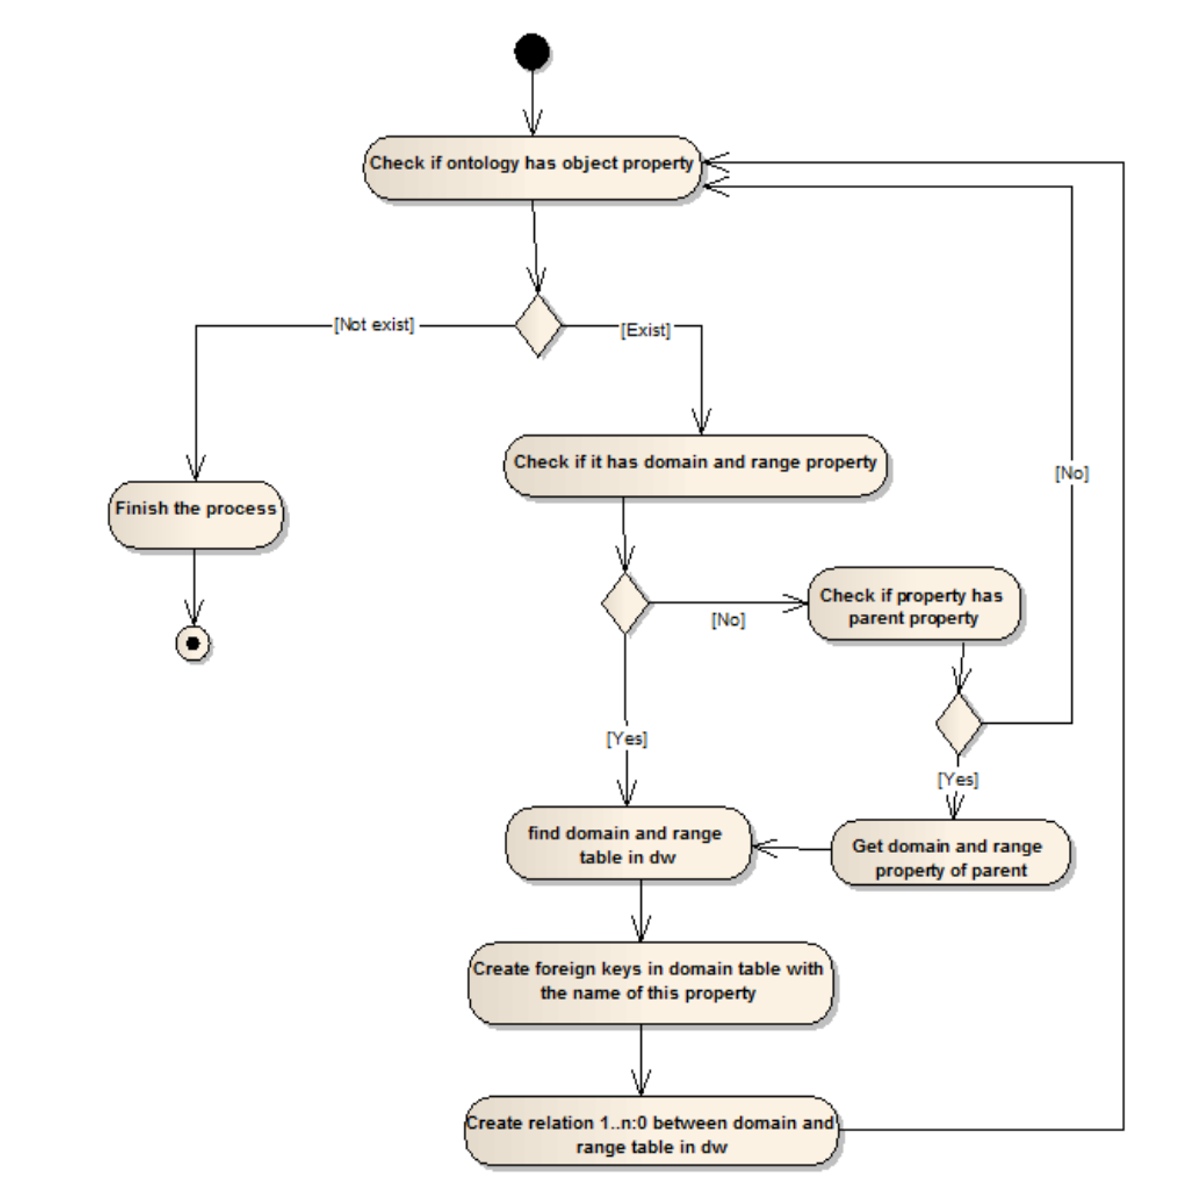
\includegraphics[scale=0.18]{object_property}
\end{center}
}
\end{frame}


\begin{frame}
\misc
{ \textbf{\Large Pasos a seguir para generar el DW}
\newline
\newline

\begin{itemize}
  \item \textbf{Creación de tablas a partir de las clases}.
  \item \textbf{Relaciones de subclase}.
  \item \textbf{Definiendo relaciones de propiedad de objetos}
  \item \textbf{Definiendo relaciones de propiedad de datos}
\end{itemize}

}
\end{frame}

\fbckg{white}
\begin{frame}
\misc
{
\begin{center}
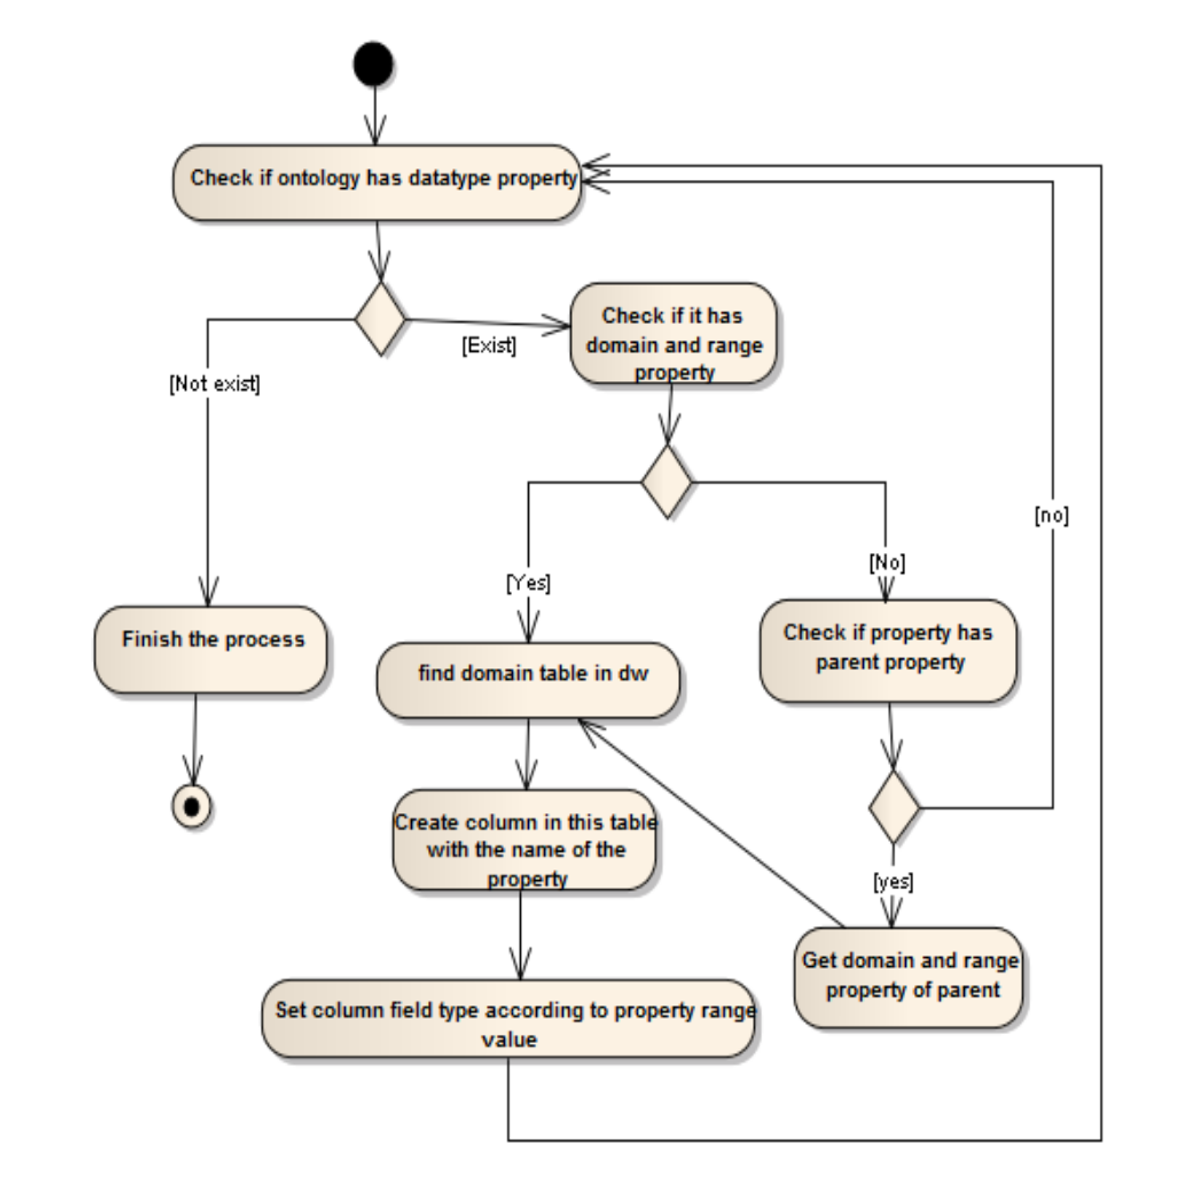
\includegraphics[scale=0.18]{data_property}
\end{center}
}
\end{frame}


\begin{frame}
\misc
{ \textbf{\Large Pasos a seguir para generar el DW}
\newline
\newline

\begin{itemize}
  \item \textbf{Creación de tablas a partir de las clases}.
  \item \textbf{Relaciones de subclase}.
  \item \textbf{Definiendo relaciones de propiedad de objetos}
  \item \textbf{Definiendo relaciones de propiedad de datos}
  \item \textbf{Insertando datos en las tablas}
\end{itemize}

}
\end{frame}

\fbckg{white}
\begin{frame}
\misc
{
\begin{center}
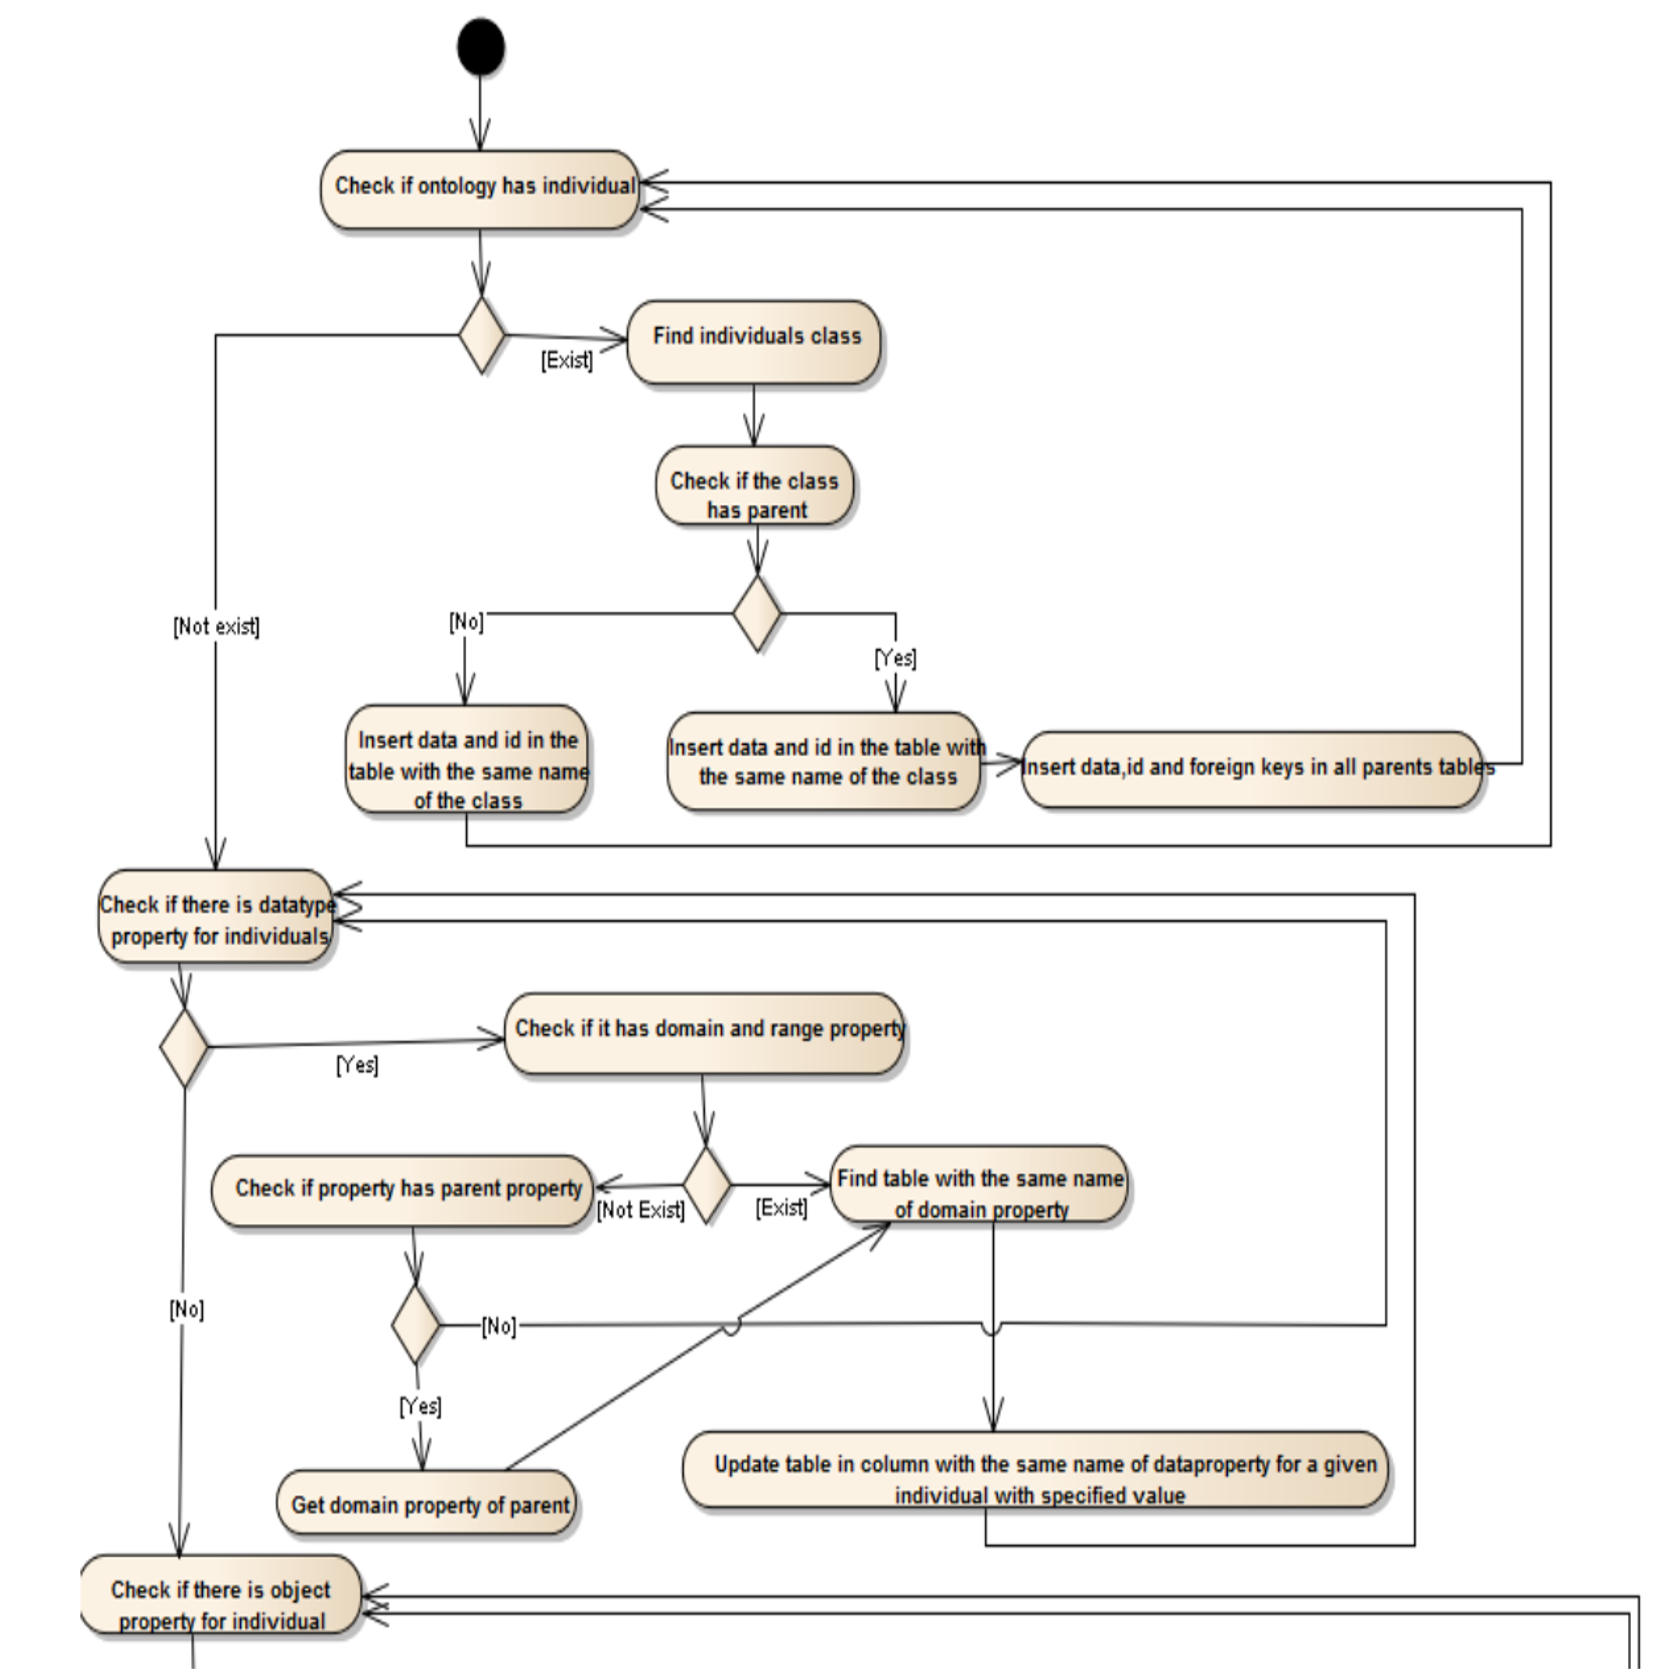
\includegraphics[scale=0.12]{inserting_data1}
\end{center}
}
\end{frame}

\fbckg{white}
\begin{frame}
\misc
{
\begin{center}
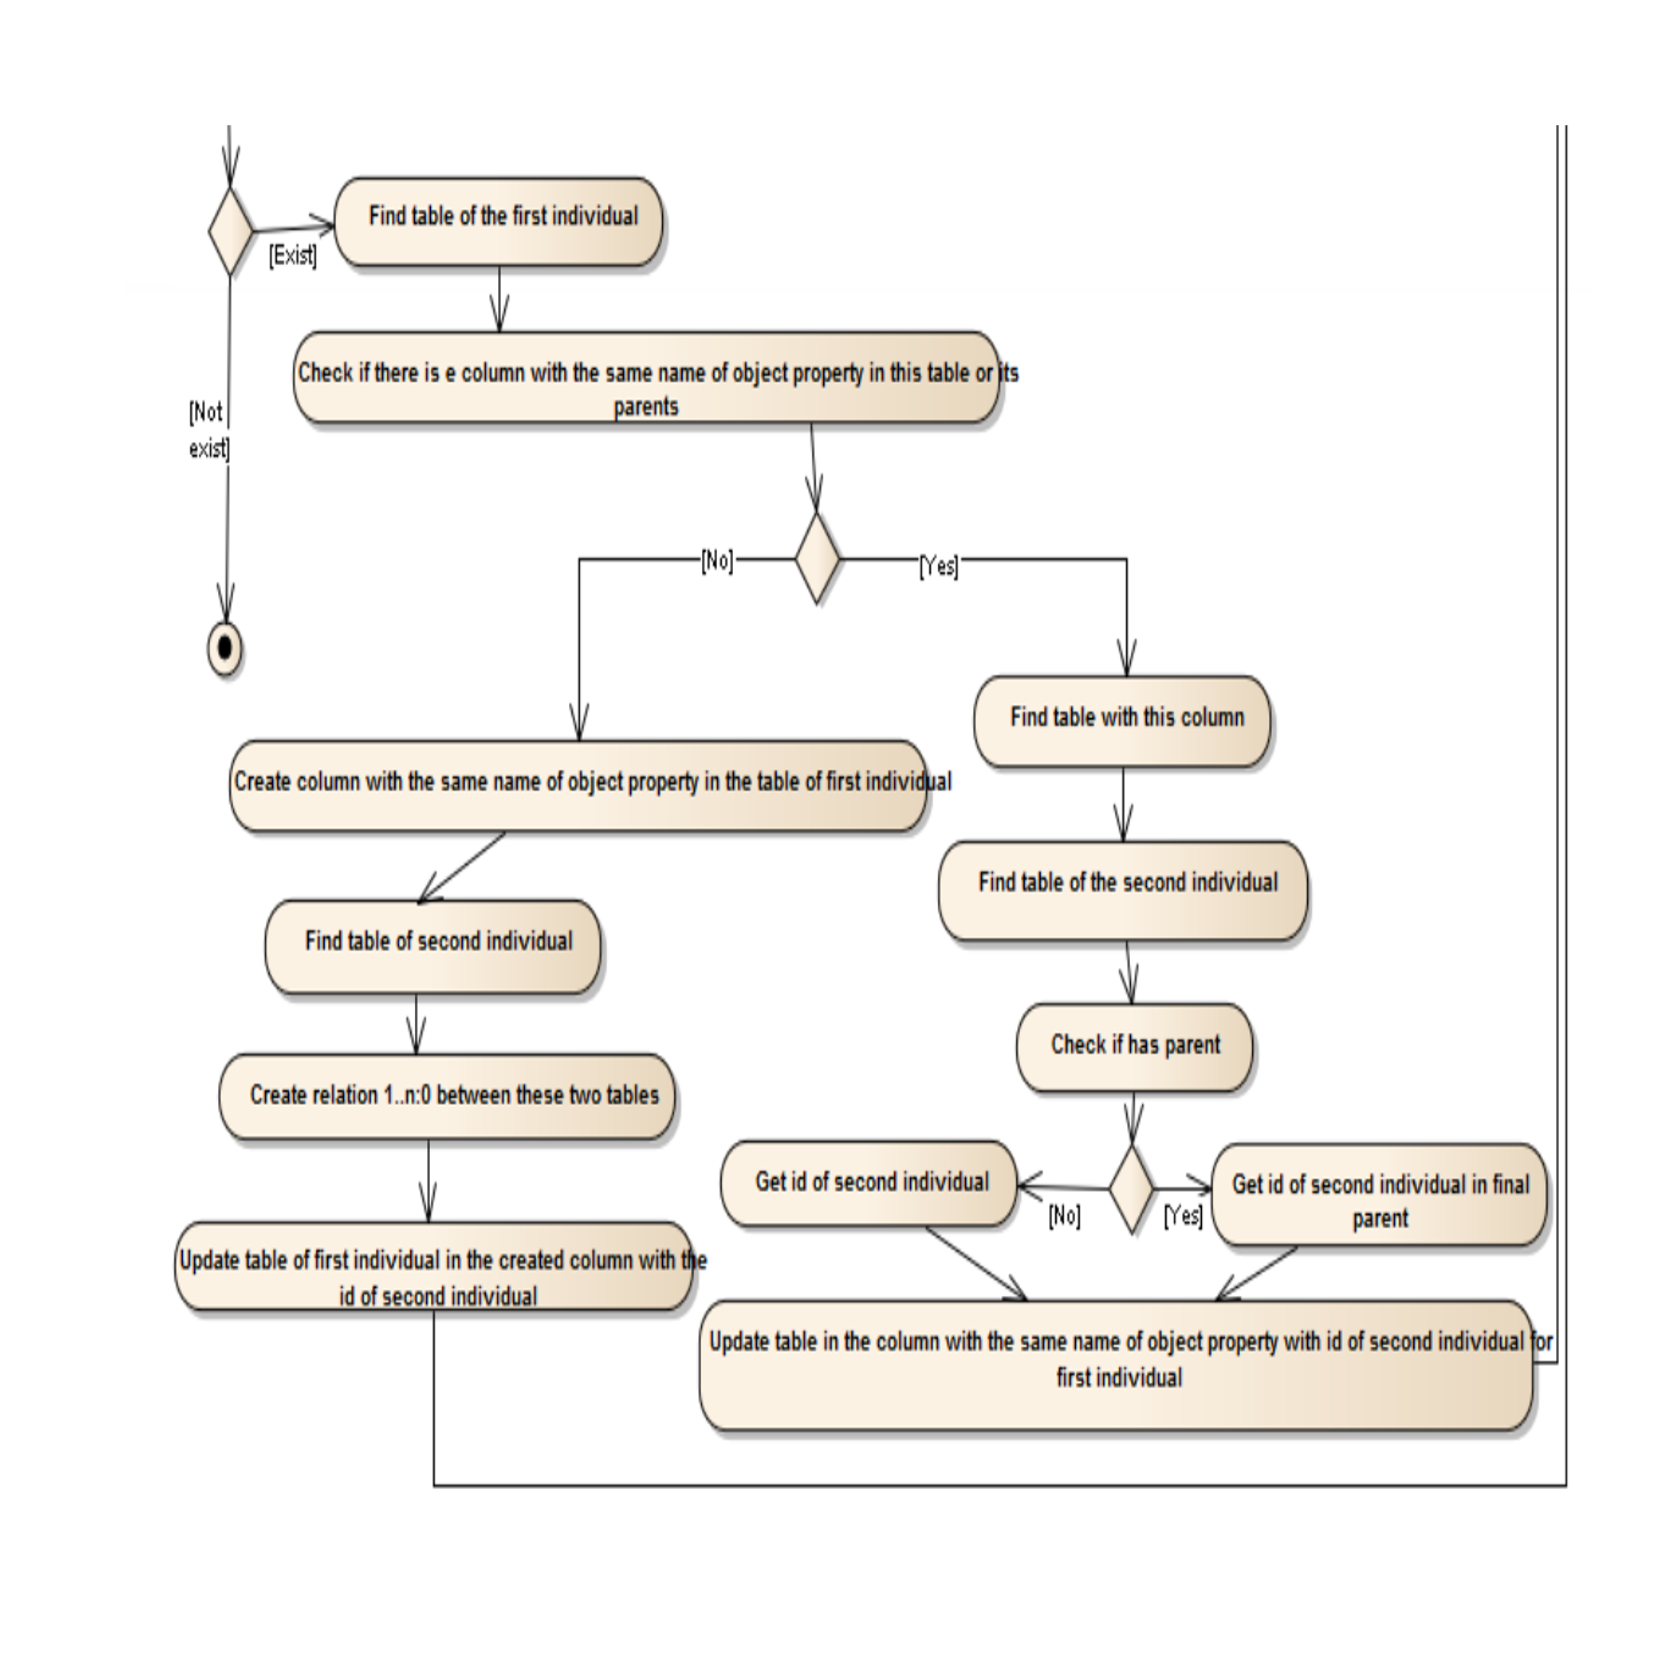
\includegraphics[scale=0.12]{inserting_data2}
\end{center}
}
\end{frame}


\fbckg{white}
\begin{frame}
\misc
{

\justifying Tomando la siguiente ontología

\begin{center}
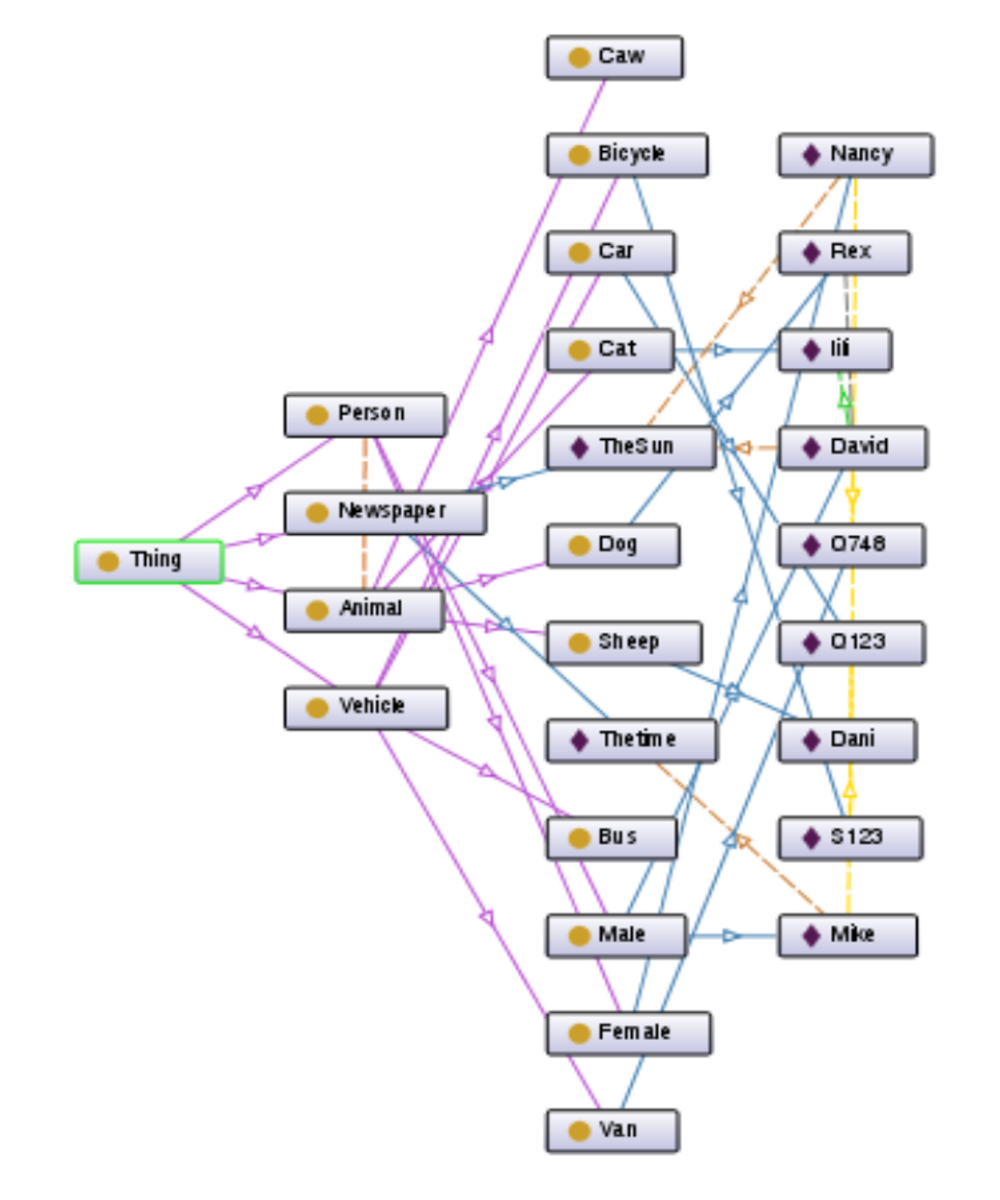
\includegraphics[scale=0.15]{ontology}
\end{center}

}
\end{frame}


\fbckg{white}
\begin{frame}
\misc
{

\justifying Obtenemos

\begin{center}
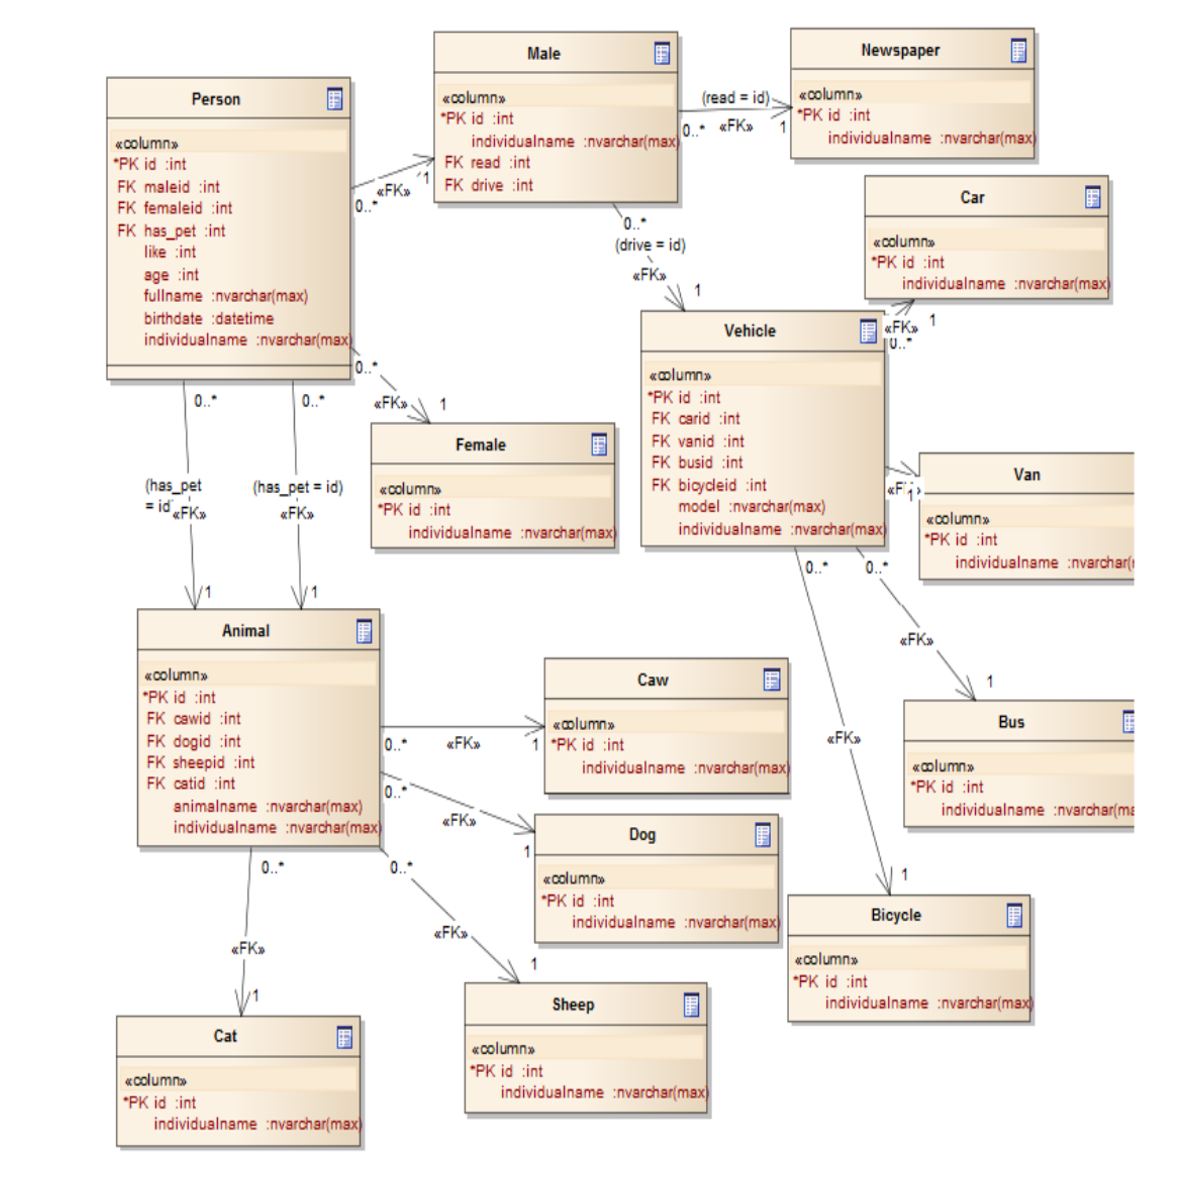
\includegraphics[scale=0.15]{owl2dw}
\end{center}

}
\end{frame}


\fbckg{white}
\begin{frame}
\pointedsl{{\Large Fuzzy Data Warehouse}}
\end{frame}

\fbckg{white}
\begin{frame}
\misc
{ \textbf{Breve repaso de lógica difusa}
\newline

\justifying \textbf{Conjunto difuso}. Un conjunto difuso $A$ en $M$, tambien llamado universo del discurso, es caracterizado por una función
$\mu_{A}(m)$, que asocia a cada elemento en $M$, un número en el intervalo $[0,1]$. Los números en el intervalo $[0,1]$ difinen la pertenencia
de un elemento $m$ al conjunto difuso A, donde 1 implica plena pertenencia, y 0 implica ninguna pertenencia.
Un conjunto difuso $A$ en $M$, puede ser representado como un conjunto de tuplas $\{ (m, \mu_{A}(m))\}$.

}
\end{frame}

\fbckg{white}
\begin{frame}
\misc
{
Una \textbf{variable lingüística} es una quintupla, $(X, T(X), G, M, F)$, definida como sigue:
\begin{itemize}
  \item $X$ es el nombre de la variable lingüística.
  \item $T(X)$, es el conjunto de términos lingüísticos de X.
  \item $G$ representa una regla sintáctica que genera el conjunto de términos lingüísticos.
  \item $M$ es el universo de discurso.
  \item $F$ es una regla semántica que define para cada término lingüístico, su significado en el sentido de un subconjunto borroso en M.
\end{itemize}

}
\end{frame}


\fbckg{white}
\begin{frame}
\misc
{
\textbf{Ejemplo}
\newline

\justifying Consideramos un conjuntos de películas, donde cada película tiene una duración específica.
Podemos definir una variable lingüística \textit{duration}, y podemos dividirla en un conjunto de términos lingüísticos {\footnotesize $\{ very\,short, short, medium, long, very\,long \}$. }

Difinimos la variable ligüística $duration$, como sigue:

{\footnotesize $(X = duration, T(X) = \{ very\,short, short, medium, long, very\,long \}, G, M = [0,200], F)$}.
}
\end{frame}

\fbckg{white}
\begin{frame}
\misc
{
\begin{center}
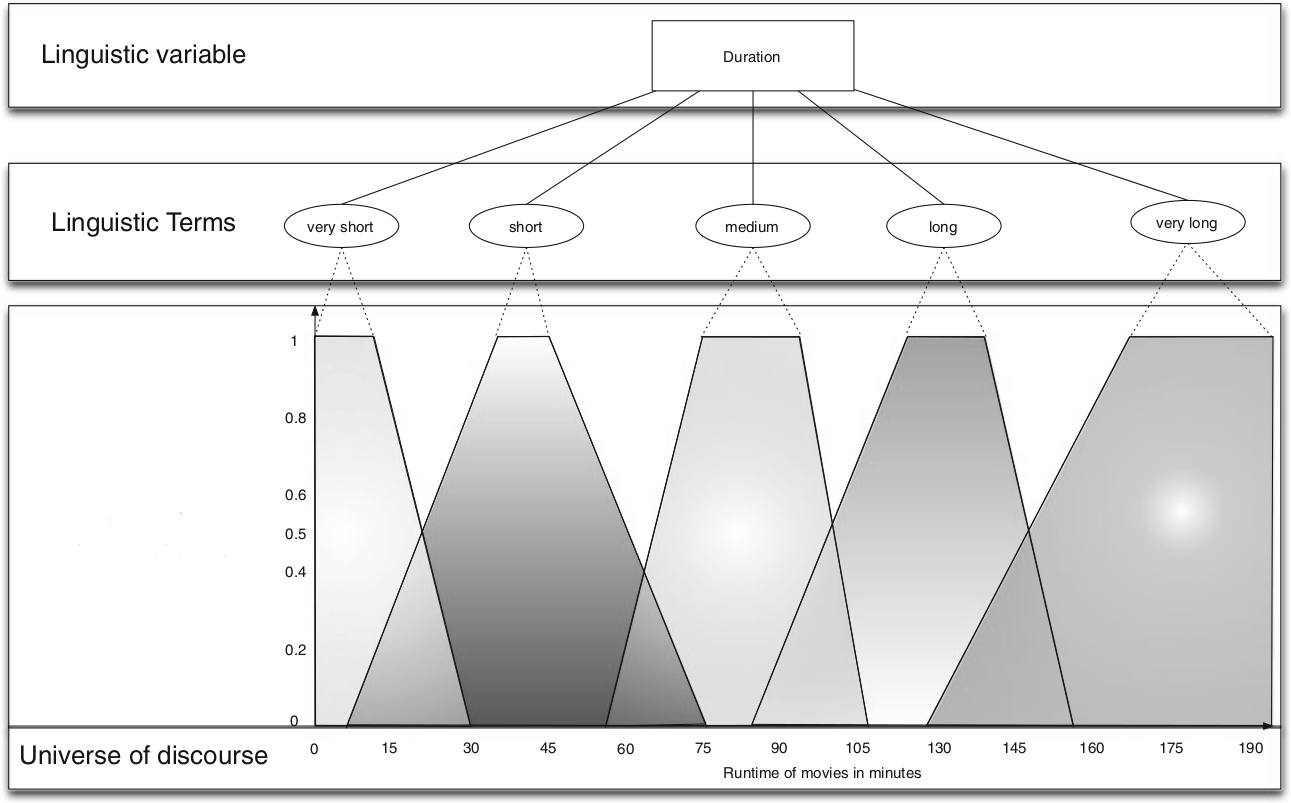
\includegraphics[scale=0.2]{fuzzy1}

Representación gráfica de la variable lingüística $duration$
\end{center}
}
\end{frame}

\fbckg{white}
\begin{frame}
\misc
{
\textbf{Conceptos básicos del modelo Fuzzy Data Warehouse}, propuesto en \cite{Fasel14}.

\begin{itemize}
%   \item \justifying \textbf{Dominio del atributo}. Al conjunto de posibles valores que puede tener el atributo de una dimensión o un hecho, se lo llama dominio de un atributo. Podemos representarlo como $Dom_{A}$.

  \item \justifying El \textbf{atributo objetivo}, lo notamos $TA$, es un atributo, de una dimensión o hecho, que quiere ser clasificado como difuso.

  \item \justifying El \textbf{atributo de pertenencia a una clase}, para un TA, es un atributo que tiene un conjunto de términos lingüísticos $T_{1},T_{2}, \ldots , T_{k}$. Lo notamos $CMA_{TA}$.
\end{itemize}
}
\end{frame}


\fbckg{white}
\begin{frame}
\misc
{
\begin{itemize}
%   \item \justifying El \textbf{grado de pertenencia}. $MD \in [0,1]$ es el grado con el que los valores del $TA$, están relacionados con los términos
% ligüísticos $T_{1},T_{2}, \ldots , T_{k}$, del $CMA_{TA}$.

  \item \justifying La \textbf{función de pertenencia}, para un término lingüístico $t$ en $CMA_{TA}$, $\mu_{t} : TA \rightarrow [0,1]$,
  es utilizada para calcular los grados de pertencia de los valores en TA, al término $t$.

  \item \justifying El \textbf{atributo grado de pertenencia}, de un TA, lo notamos $MDA_{TA}$, tiene el conjunto de grados de pertencia del TA,
  para cada término lingüístico en $CMA_{TA}$.
\end{itemize}
}
\end{frame}

\fbckg{white}
\begin{frame}
\misc
{
\begin{itemize}
  \item \justifying La \textbf{tabla de clasificación fuzzy}, $FCTA$, es un tabla con dos atributos, los términos ligüísticos y sus identificadores.
  
  Es decir, $FCT_{TA} = \{ ID, CMA_{TA} \}$.
  \item \justifying La \textbf{tabla de pertenencia fuzzy}, $FMT$, es una tabla que almacena los valores que representan el grado en que un valor está relacionado con un término lingüístico.
  
  Es decir, $FMT_{TA} = \{ ID, ID \, de \, TA, ID \, de \, CMA_{TA}, MDA_{TA} \}$.
  
  \item \justifying Un \textbf{modelo Fuzzy Data Warehouse}, es un conjunto de tablas, $FDW = \{Dim, Fact, FCT_{TA}, FMT_{TA} \}$.
\end{itemize}
}
\end{frame}

\fbckg{white}
\begin{frame}
\misc
{

\begin{center}
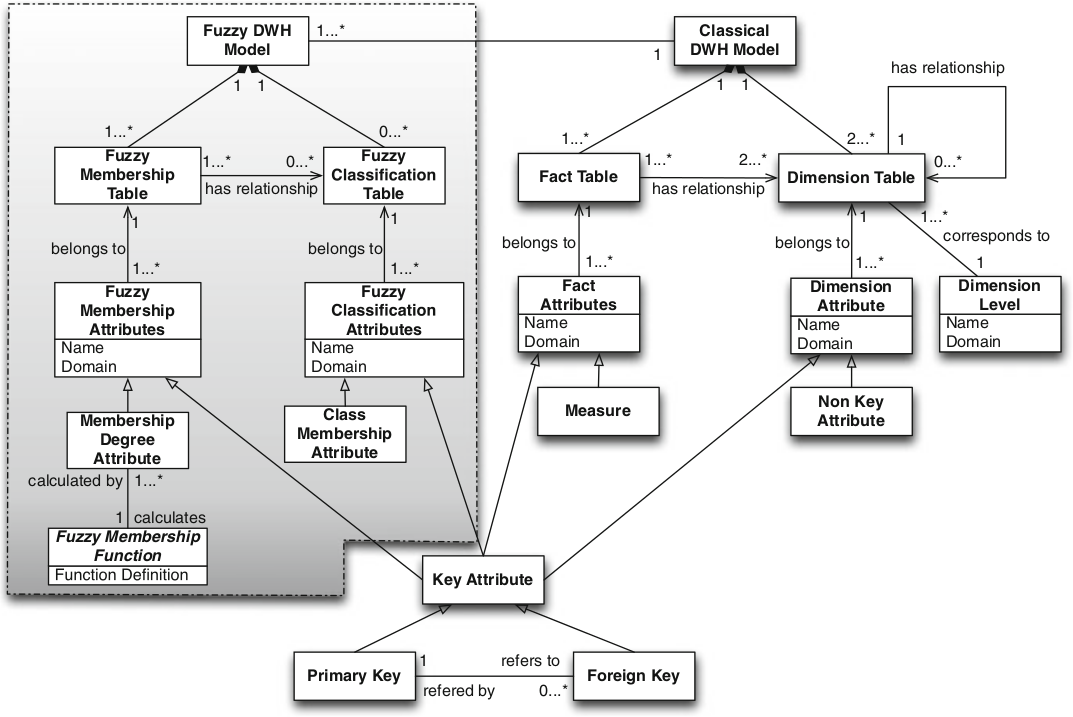
\includegraphics[scale=0.25]{fuzzy2}

El meta modelo Fuzzy Data Warehouse
\end{center}

}
\end{frame}

\fbckg{white}
\begin{frame}
\misc
{
\justifying Para una comprensión más certera de los valores numéricos, los usuarios requieren una interpretación en términos significativos, no numéricos.
Una solución a esto es el uso de un enfoque fuzzy.

Por ejemplo, en \cite{Fasel09} se propone un Fuzzy Data Warehouse para un sistema de análisis web, donde se demuestra que las medidas para un análisis web no siempre son fáciles de interpretar, pues no es posible contar las visitas de distintos usuarios con precisión.
El concepto difuso sobre las visitas a páginas web proporciona una clasificación más precisa que la clasificación en bruto.
}
\end{frame}

\fbckg{white}
\begin{frame}
\misc
{
\textbf{Beneficios del concepto}
\newline

Las principales ventajas de este enfoque son los siguientes:
\begin{itemize}
  \item Los datos pueden ser analizados en forma difusa y no difusa.
  \item El modelo puede ser utilizado para el modelado de nuevos DWs, o aplicado a uno ya existente.
\end{itemize}
}
\end{frame}


\fbckg{white}
\begin{frame}
\misc
{ Bibliografía:

\printbibliography
}
\end{frame}

\end{document}
